\section{Model of the Memory}
This section presents the model for the system memory. Its purpose is to
model reading and writing times.

\label{sec:model:memory}
\begin{figure}[hbt!]
\begin{center}
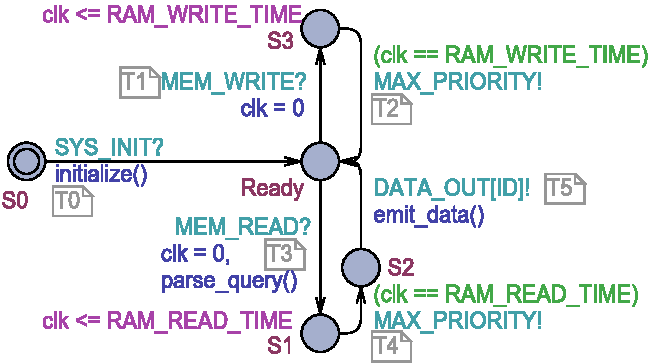
\includegraphics[width=0.5\textwidth]{\chapterdirectory/figure/MemoryCTRL.pdf}
\end{center}
\caption{Automaton of the Memory Controller}
\label{fig:UPPAAL:MemoryCTRL}
\end{figure}

Figure~\ref{fig:UPPAAL:MemoryCTRL} shows the automaton corresponding to the
memory. It uses the following variables:
\paragraph{Clocks \& Variables for System Memory}
\begin{itemize}
\item
   \lstinline!clk! is the clock controlling periods of inactivity that
   emulate either reading or writing times.
\item
   \lstinline!msg! is a copy of the message that must be sent once the waiting
   period is over.
\end{itemize}
%\end{varandclocks}

The memory controller automaton starts in the $S_0$ location.

\paragraph{Transitions for System Memory}
\begin{description}
\item[$S_0 \automatatransitiontrace{T_{0}}{} \texttt{Ready}$]
   Upon synchronization on the \textbf{SYS\_INIT} broadcast channel,
   \lstinline!msg! takes an arbitrary default value. The memory controller is
   then ready to synchronize with the coherence manager.

\item[$\texttt{Ready} \automatatransitiontrace{T_{1}}{} S_3$]
   Upon synchronization on the \textbf{MEM\_WRITE} channel, \lstinline!clk!
   is set to zero in order to prepare an inactivity period corresponding to
   a \writeact{}.

\item[$S_3 \automatatransitiontrace{T_{2}}{} \texttt{Ready}$]
   As soon as the \lstinline!RAM_WRITE_TIME! period has elapsed, the memory
   controller becomes available to the coherence manager again.

\item[$\texttt{Ready} \automatatransitiontrace{T_{3}}{} S_1$]
   Upon synchronization on the \textbf{MEM\_READ} channel, \lstinline!clk!
   is set to zero in order to prepare an inactivity period corresponding to
   a \readact{}. Additionally, the message held in the information sharing
   global variable is stored in \lstinline!msg! so that it can be sent once the
   inactivity period is over.

\item[$S_1 \automatatransitiontrace{T_{4}}{} S_2$]
   As soon as the \lstinline!RAM_READ_TIME! period has elapsed, the memory
   controller enters a location from which it will attempt to send the message
   held in \lstinline!msg!.

\item[$S_2 \automatatransitiontrace{T_{5}}{} \texttt{Ready}$]
   Upon synchronization on the \textbf{DATA\_OUT} sub-channel corresponding to
   the memory controller's component ID, the value of \lstinline!msg! is put in
   the information sharing global variable in order to have it be received by
   the data FIFO automaton, which will add it to its outgoing data message
   queue.

   Once this is done, the memory controller is once again available for the
   coherence manager to synchronize with.
\end{description}
